\documentclass[10pt,letterpaper]{article}
\usepackage[latin1]{inputenc}
\usepackage{amsmath}
\usepackage{amsfonts}
\usepackage{amssymb}
\usepackage{graphicx}
\usepackage[margin=1in]{geometry}
\usepackage{listings}
\usepackage{float}
\usepackage{fancyhdr}
\pagestyle{fancy}
\lhead{\today}
\chead{Project 2}
\rhead{Tan, Zhou}
%\usepackage[margin=1in]{geometry}
\usepackage{color} %red, green, blue, yellow, cyan, magenta, black, white
\definecolor{mygreen}{RGB}{28,172,0} % color values Red, Green, Blue
\definecolor{mylilas}{RGB}{170,55,241}

\newcommand{\ssbracket}[2]{#1^{(#2)}}

\author{Hao Hui Tan(999741711, tanstev1)\\Kyle Zhou (1000959732, zhoukyle)}
\title{CSC411H1S Project 2}
\begin{document}
	\lstset{language=Python,%
		%basicstyle=\color{red},
		breaklines=true,%
		%morekeywords={matlab2tikz},
		keywordstyle=\color{blue},%
		morekeywords=[2]{1}, keywordstyle=[2]{\color{black}},
		identifierstyle=\color{black},%
		stringstyle=\color{mylilas},
		commentstyle=\color{mygreen},%
		showstringspaces=false,%without this there will be a symbol in the places where there is a space
		numbers=left,%
		numberstyle={\tiny \color{black}},% size of the numbers
		numbersep=9pt, % this defines how far the numbers are from the text
		emph=[1]{for,end,break},emphstyle=[1]\color{red}, %some words to emphasise
		%emph=[2]{word1,word2}, emphstyle=[2]{style},
		caption=\lstname,
	}

	\maketitle
	\newpage
	\textbf{Important Note:} We have tested our faces and deepfaces code on CDF machines with GPU supported (using Nvidia Cuda). The code will run significantly slower on machines with no GPUs.
	\section{Part 1}
	Each of the digits in the training and test sets, respectively, seem to look very similar, except that some may have different brightnesses.
	All of the digits are centered in a 28x28px frame, and they are anti-aliased.
	\begin{figure}[H]
		\minipage{0.48\textwidth}
		\centering
		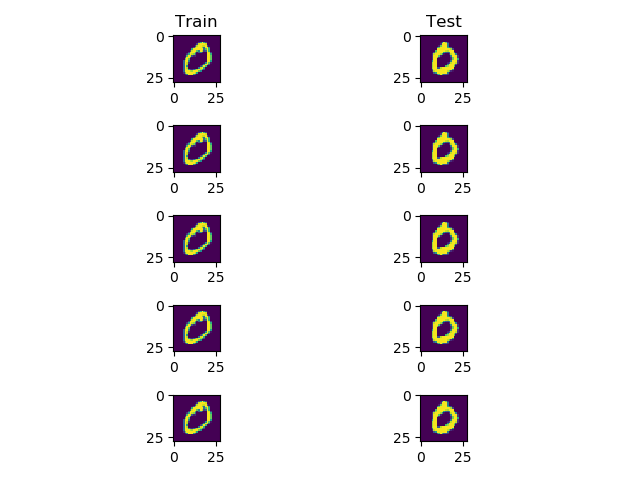
\includegraphics[width=\linewidth]{imgs/digit-0}
		\caption{Ten selected samples of the number 0 from the Training and Test sets}
		\label{fig:digit-0}
		\endminipage\hfill
		\minipage{0.48\textwidth}
		\centering
		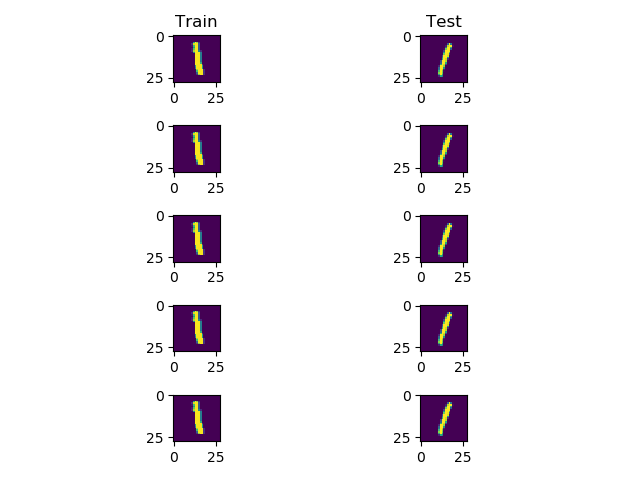
\includegraphics[width=\linewidth]{imgs/digit-1}
		\caption{Ten selected samples of the number 1 from the Training and Test sets}
		\label{fig:digit-1}
		\endminipage\hfill
	\end{figure}
	\begin{figure}[H]
		\minipage{0.48\textwidth}
		\centering
		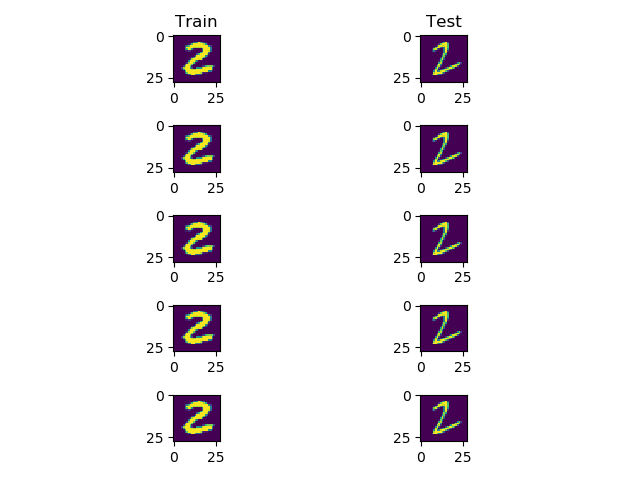
\includegraphics[width=\linewidth]{imgs/digit-2}
		\caption{Ten selected samples of the number 2 from the Training and Test sets}
		\label{fig:digit-2}
		\endminipage\hfill
		\minipage{0.48\textwidth}
		\centering
		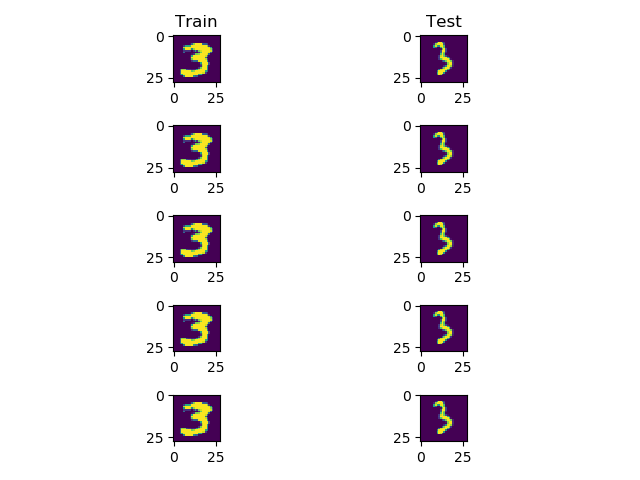
\includegraphics[width=\linewidth]{imgs/digit-3}
		\caption{Ten selected samples of the number 3 from the Training and Test sets}
		\label{fig:digit-3}
		\endminipage\hfill
	\end{figure}
	\begin{figure}[H]
		\minipage{0.48\textwidth}
		\centering
		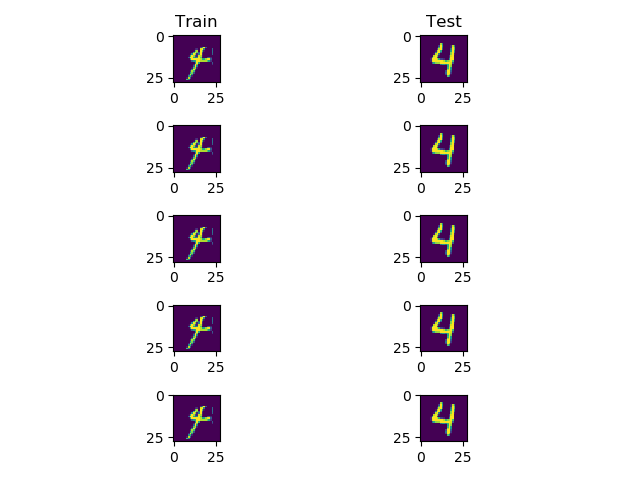
\includegraphics[width=\linewidth]{imgs/digit-4}
		\caption{Ten selected samples of the number 4 from the Training and Test sets}
		\label{fig:digit-4}
		\endminipage\hfill
		\minipage{0.48\textwidth}
		\centering
		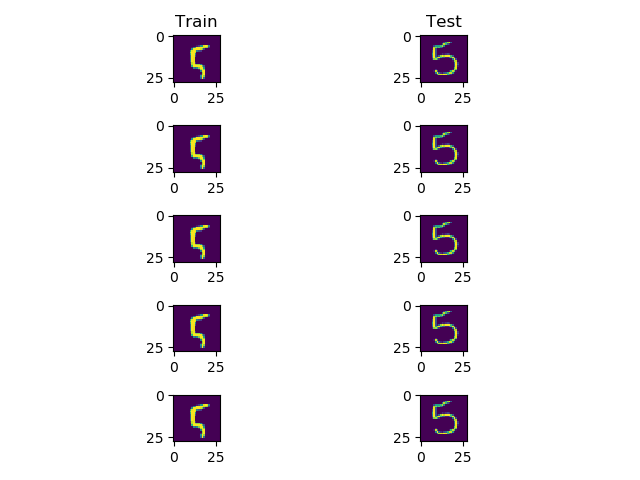
\includegraphics[width=\linewidth]{imgs/digit-5}
		\caption{Ten selected samples of the number 5 from the Training and Test sets}
		\label{fig:digit-5}
		\endminipage\hfill
	\end{figure}
	\begin{figure}[H]
		\minipage{0.48\textwidth}
		\centering
		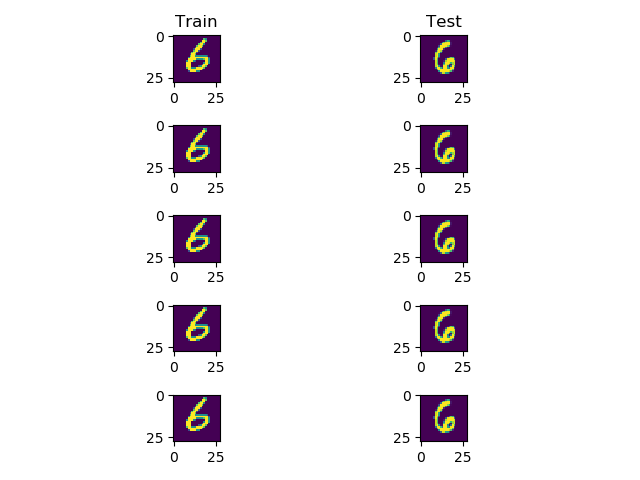
\includegraphics[width=\linewidth]{imgs/digit-6}
		\caption{Ten selected samples of the number 6 from the Training and Test sets}
		\label{fig:digit-6}
		\endminipage\hfill
		\minipage{0.48\textwidth}
		\centering
		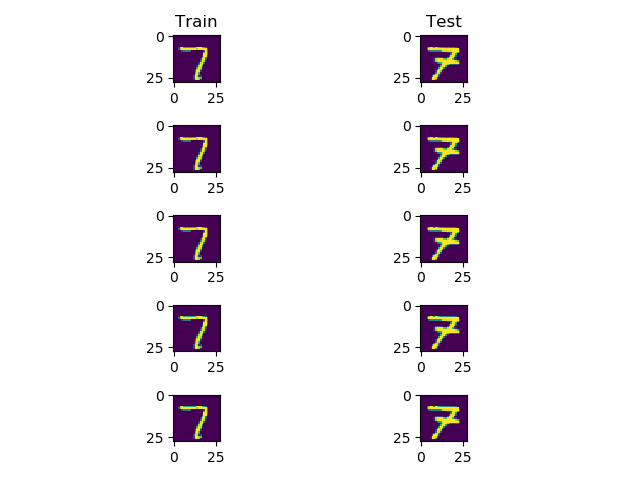
\includegraphics[width=\linewidth]{imgs/digit-7}
		\caption{Ten selected samples of the number 7 from the Training and Test sets}
		\label{fig:digit-7}
		\endminipage\hfill
	\end{figure}
	\begin{figure}[H]
		\minipage{0.48\textwidth}
		\centering
		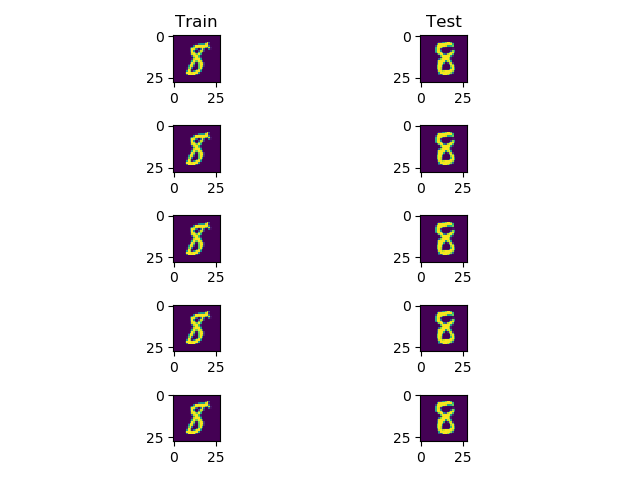
\includegraphics[width=\linewidth]{imgs/digit-8}
		\caption{Ten selected samples of the number 8 from the Training and Test sets}
		\label{fig:digit-8}
		\endminipage\hfill
		\minipage{0.48\textwidth}
		\centering
		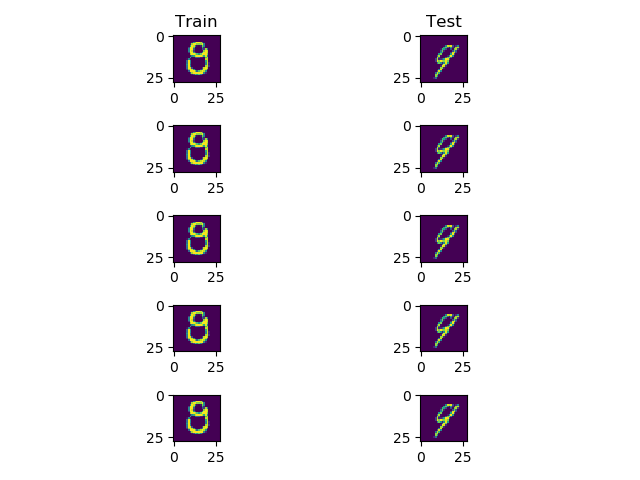
\includegraphics[width=\linewidth]{imgs/digit-9}
		\caption{Ten selected samples of the number 9 from the Training and Test sets}
		\label{fig:digit-9}
		\endminipage\hfill
	\end{figure}

	\section{Part 2}
	\begin{lstlisting}
	def compute_network(x_input, weights, b):
	"""
	Returns the linear combination of x_input matrix and weights matrix plus b the bias unit vector  (part 2)
	"""
	return np.dot(weights.T, x_input) + b
	\end{lstlisting}
	\section{Part 3}
	\subsection*{Part 3a}
	\[p_i = \frac{e^{o_i}}{\sum_j e^{o_j}}\]
	\begin{align*}
	\frac{\partial p_i}{\partial o_i} &= \frac{e^{o_i}\sum_j e^{o_j} - (e^{o_i})^2}{(\sum_j e^{o_j})^2} & \text{By the Quotient Rule}\\
	&= \frac{e^{o_i}}{\sum_j e^{o_j}} - \frac{(e^{o_i})^2}{(\sum_j e^{o_j})^2}\\
	&= \frac{e^{o_i}}{\sum_j e^{o_j}}\left(1 - \frac{e^{o_i}}{\sum_j e^{o_j}}\right) & \text{Substituting } p_i\ \text{back in}
	\end{align*}
	\[C = -\sum_j y_j \log p_j\]
	\begin{align*}
	\frac{\partial C}{\partial o_i} &= \sum_j \frac{\partial C}{\partial p_j} \frac{\partial p_j}{\partial o_i} = p_i - y_i % todo: understand this
	\end{align*}
	Since we want to find the gradient of the cost function with respect to the weights, we must also compute \(\frac{\partial o_j}{\partial w_{ij}}\)
	\[\frac{\partial o_j}{\partial w_{ij}} = x_i\]
	\[\text{Since }o_i = \sum_j w_{ji} x_j + b_i\]
	Thus, by the multivatiate chain rule, we find that
	\[\frac{\partial C}{\partial w_{ij}} =\frac{\partial C}{\partial o_j} \times \frac{\partial o_j}{\partial w_{ij}}\]
	\[= (p_i - y_i)x_i\]
	\subsection*{Part 3b}
	Listing \ref{lst:gradient} contains the code for computing the gradient in vectorized form.

	We computed the finite differences matrix over ten images from the training set (one per digit).
	We then computed the difference matrix between the gradient and finite differences matrices, and we found that the max difference at any index in the matrix is 0.006916014765721457 given an h-value of $10^{-12}$, which is quite small.

	Thus, we know that our gradient function is correctly implemented.\\

	See Listing \ref{lst:finitediff} for the code we used to compute this matrix.
	\begin{lstlisting}[label=lst:gradient]
def compute_gradient(p_i, y_i, x_matrix):
    """
    number of categories = 10
    p_i (10 x m) is softmax, y_i (10 x m) is the ground truth, x_matrix (784 x m) is the matrix of pixels of images
    The resulting matrix should be 10 x 784
    """
    return np.dot(p_i - y_i, x_matrix.T)
	\end{lstlisting}
	\begin{lstlisting}[label=lst:finitediff]
def finite_difference(h=0.000000000001, initial_weights_coefficient=0, m=10):
    """weights are 784 x 10, x_matrix is the 784 x 10 image input matrix
    (number of digits, we are trying to classify from 0-9),
    ground truth is 10 x 10 where m is number of sample images.

    Return the gradient matrix, the finite difference matrix and the difference matrix between them
    """
    # Build up the x_matrix -> 784 x m and the y ground truths
    # Get 10 images
    imgs = []
    y_ground_truths = np.identity(10)
    for i in xrange(10):
        img = M['train{}'.format(i)][0]
        imgs.append(img)

    x_matrix = np.vstack(imgs).T

    b = np.ones(10)
    #b = np.zeros(10)

    # Build up the weights matrix
    initial_weights = []
    for i in range(m):
        initial_weights_row = initial_weights_coefficient * np.ones(x_matrix.shape[0])
        initial_weights.append(initial_weights_row)
    initial_weights = np.vstack(initial_weights)
    initial_weights = initial_weights.T
    initial_weights_copy = initial_weights.copy()

    # gradient dimension is 10 x 784
    gradient = compute_gradient(softmax(compute_output(initial_weights, x_matrix, b)), y_ground_truths, x_matrix)
    lst_finite_difference = []

    # lst_finite_difference dimension is 10 x 784
    for row_idx in range(784):
        lst_row = []
        for column_idx in range(10):
            cost_function_original = cost_f(initial_weights, x_matrix, b, y_ground_truths)
            initial_weights_copy[row_idx][column_idx] = initial_weights_copy[row_idx][column_idx] + h
            cost_function_added_h = cost_f(initial_weights_copy, x_matrix, b, y_ground_truths)
            finite_difference = (cost_function_added_h - cost_function_original) / h
            lst_row.append(finite_difference)
            initial_weights_copy = initial_weights.copy()
        lst_finite_difference.append(lst_row)
    return gradient, lst_finite_difference, gradient - array(lst_finite_difference).T
	\end{lstlisting}
	\section{Part 4}
	For part 4 gradient descent, we initialize the weights to be a matrix of 0.001 and we choose the learning rate to be 0.0000001. The maximum iteration limit on the gradient descent is 10000.
	See Figure \ref{fig:part4-learncurve} is the plot of the learning curve:
	\begin{figure}[H]
		\centering
		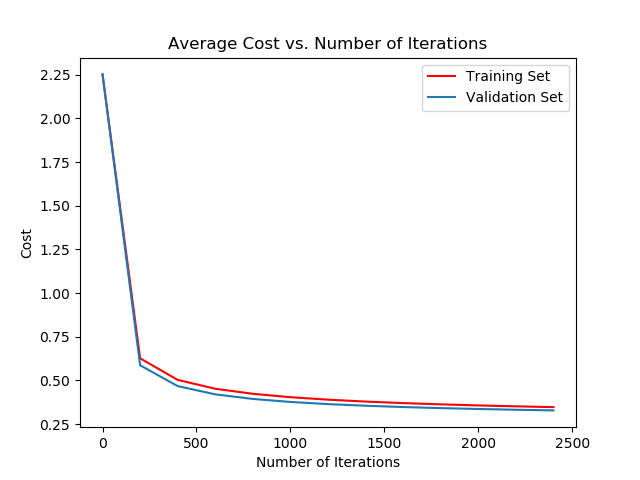
\includegraphics[width=\linewidth]{part_4_validation_training_plot.png}
		\caption{Learning curve of the Neural Network Without Momentum}
		\label{fig:part4validationtrainingplot}
	\end{figure}

	Below is a visualization of the weights that were fed into each output.

	\begin{figure}[H]
		\begin{minipage}{0.48\textwidth}
			\centering
			
\includegraphics[width=0.7\linewidth]{imgs/weights_visual_0.png}
			\caption{Output 0}
			\label{fig:part5-0}
		\end{minipage}
		\begin{minipage}{0.48\textwidth}
			\centering
			
\includegraphics[width=0.7\linewidth]{imgs/weights_visual_1.png}
			\caption{Output 1}
			\label{fig:part5-1}
		\end{minipage}
	\end{figure}

	\begin{figure}[H]
		\begin{minipage}{0.48\linewidth}
			\centering
			
\includegraphics[width=0.7\linewidth]{imgs/weights_visual_2.png}
			\caption{Output 2}
			\label{fig:part5-2}
		\end{minipage}
		\begin{minipage}{0.48\linewidth}
			\centering
			
\includegraphics[width=0.7\linewidth]{imgs/weights_visual_3.png}
			\caption{Output 3}
			\label{fig:part5-3}
		\end{minipage}
	\end{figure}

	\begin{figure}[H]
		\begin{minipage}{0.48\linewidth}
		    \centering
			
\includegraphics[width=0.7\linewidth]{imgs/weights_visual_4.png}
			\caption{Output 4}
			\label{fig:part5-4}
		\end{minipage}
		\begin{minipage}{0.48\linewidth}
		    \centering
			
\includegraphics[width=0.7\linewidth]{imgs/weights_visual_5.png}
			\caption{Output 5}
			\label{fig:part5-5}
		\end{minipage}
	\end{figure}

	\begin{figure}[H]
		\begin{minipage}{0.48\linewidth}
		    \centering
			
\includegraphics[width=0.7\linewidth]{imgs/weights_visual_6.png}
			\caption{Output 6}
			\label{fig:part5-6}
		\end{minipage}
		\begin{minipage}{0.48\linewidth}
		    \centering
			
\includegraphics[width=0.7\linewidth]{imgs/weights_visual_7.png}
			\caption{Output 7}
			\label{fig:part5-7}
		\end{minipage}
	\end{figure}

	\begin{figure}[H]
		\begin{minipage}{0.48\linewidth}
		    \centering
			
\includegraphics[width=0.7\linewidth]{imgs/weights_visual_8.png}
			\caption{Output 8}
			\label{fig:part5-8}
		\end{minipage}
		\begin{minipage}{0.48\linewidth}
		    \centering
			
\includegraphics[width=0.7\linewidth]{imgs/weights_visual_9.png}
			\caption{Output 9}
			\label{fig:part5-9}
		\end{minipage}
	\end{figure}


	\section{Part 5}
	Here is the learning curve with momentum:

	\begin{figure}[H]
	    \centering
		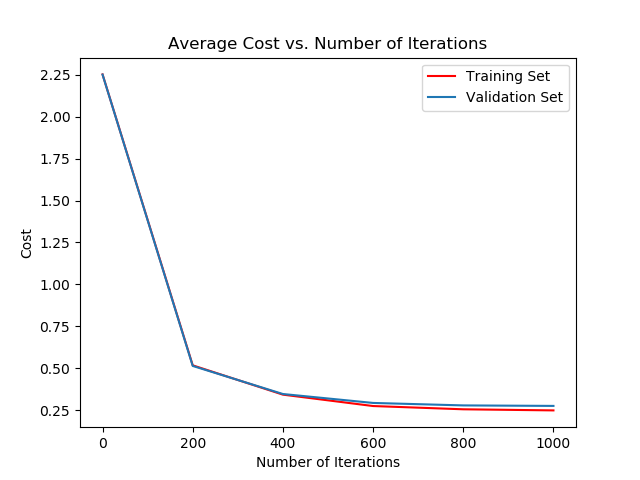
\includegraphics[width=1.0\linewidth]{part_5_validation_training_plot.png}
		\caption{Learning Curve with Momentum}
		\label{fig:part5}
	\end{figure}

	If we compare this plot with the gradient descent learning curve without momentum graph in part 4, we can see that the cost decreases faster in this graph where momentum is used. For instance, at 2000 iterations, the cost is at or below 0.25 for gradient descent with momentum while the cost is greater that 0.25 for gradient descent without momentum.
	This is the new code that we wrote that uses momentum for gradient descent.
	\begin{lstlisting}
    def grad_descent_momentum(f, df, x, y, init_t, alpha, b, max_iter=10000, momentum=0.99):
        """
        Computes weights via gradient descent
        :param f: Cost function
        :param df: Gradient of the cost function
        :param x: Inputs
        :param y: Ground Truth
        :param init_t: Initial Weights
        :param alpha: Learning Rate
        :param max_iter: Max number of iterations
        :return: Vector/Matrix of weights
        """
        intermediate_weights = {}
        EPS = 1e-5   #EPS = 10**(-5)
        prev_t = init_t-10*EPS
        t = init_t.copy()
        iter = 0
        v = 0
        while norm(t - prev_t) >  EPS and iter < max_iter:
            prev_t = t.copy()
            v = (momentum * v) + alpha*df(x, y, t, b)
            t = t - v
            if iter % 200 == 0:
                print "Iter", iter
                # print "x = (%.2f, %.2f, %.2f), f(x) = %.2f" % (t[0], t[1], t[2], f(x, y, t))
            print "Gradient: ", df(x, y, t, b), "\n"

            if iter % 2000 == 0:
                intermediate_weights[iter] = t
            iter += 1
        return t, intermediate_weights
	\end{lstlisting}
	\section{Part 6}
	\subsection*{Part 6a}
	\begin{figure}[H]
		\centering
		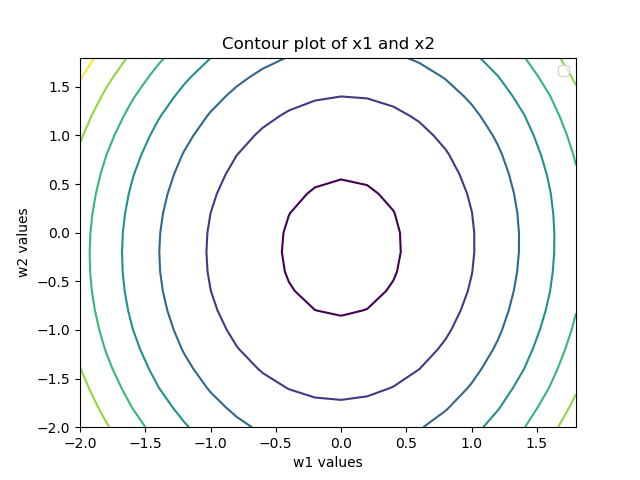
\includegraphics[width=0.7\linewidth]{part_6a_contour_plot}
		\caption{Contour Plot for the Cost Function}
		\label{fig:part6contourplot}
	\end{figure}

	\subsection*{Part 6b}
	\begin{figure}[H]
		\centering
		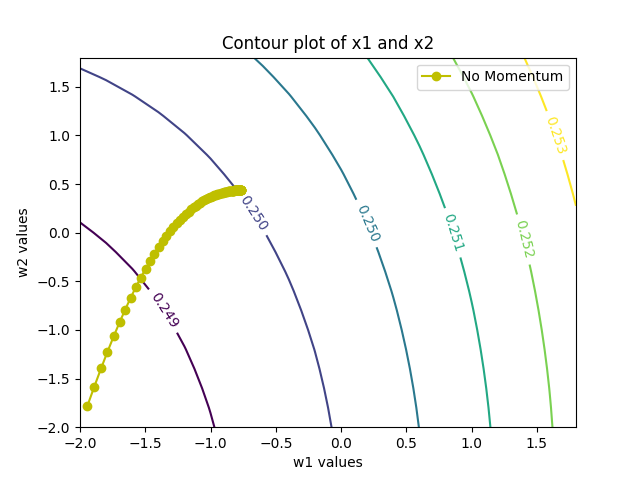
\includegraphics[width=\linewidth]{part6_contour_plot_with_trajectory-nomomentum}
		\caption{Trajectory plot of gradient descent without momentum}
		\label{fig:part6contourplotwithtrajectory-nomomentum}
	\end{figure}
	\subsection*{Part 6c}
	\begin{figure}[H]
		\centering
		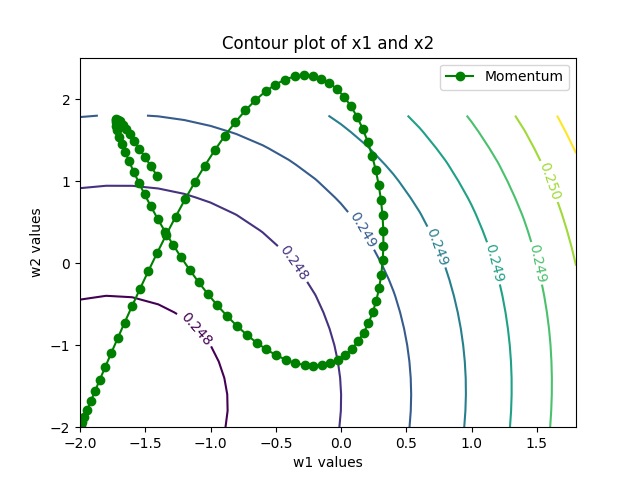
\includegraphics[width=\linewidth]{part6_contour_plot_with_trajectory-099momentum}
		\caption{Trajectory plot of gradient descent with momentum}
		\label{fig:part6contourplotwithtrajectory-099momentum}
	\end{figure}
	\subsection*{Part 6d}
    The trajectory that gradient descent without momentum takes is more stable and constant than the gradient descent with momentum. The trajectory that gradient descent with momentum takes is trying to go in one direction due to the momentum coefficient and it is harder for the algorithm to change the trajectory's course as the momentum coefficient speeds up gradient descent in the direction it is going. At around (-1.6, -0,7) we can see that the gradient descent with momentum's trajectory is tangential to the trajectory without momentum and that the momentum coefficient just keeps the trajectory going in that direction while the algorithm tries to decelerate it.
	\subsection*{Part 6e}
	When we choose weights that are initially 0s (which represents the black portion of the image) for $w_1$ and $w_2$, momentum will not help because multiplying the momentum coefficient by values near 0 will not speed up the gradient descent process much. The $x_1$ and $x_2$ initial values we used are non-zero values which works well in producing a good visualization.
	\begin{figure}[H]
		\centering
		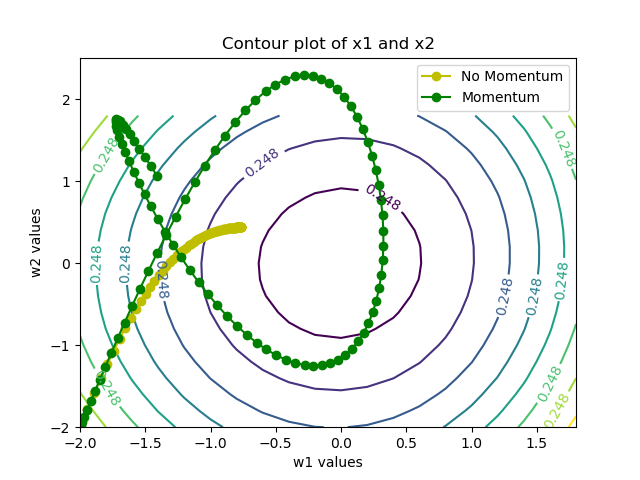
\includegraphics[width=\linewidth]{part6_contour_plot_with_trajectory}
		\caption{Trajectory plot of gradient descent with and without momentum}
		\label{fig:part6contourplotwithtrajectory}
	\end{figure}

	\section{Part 7}
	Since we are building up the gradient from cached and pre-calculated gradients using the chain rule in back-propagation,
	\[   \frac{\partial C}{\partial w_{nk}} = \frac{\partial C}{\partial h_{n}} \frac{\partial h_{n}}{\partial w_{nk}}  \]

	where h is the hidden layer at n.
	Let K be the number of neurons at each layer. Let I be the number inputs going into the layer.
	Let N be the number of layers in the neural network. If we calculate the gradient w.r.t to each weight, we assume the matrices in the matrix multiplication to be K x I matrices so each matrix multiplication would take O(KI) runtime. Since we are not caching the intermediate values in the vanilla computation of the gradients, we have to re-compute (i.e do matrix multiplication for previous layers) the values of the previous layers again. So the run-time for this would be O($(KI)^{2N}$) as we have to recompute the previous values again at each layer. In back-propagation, since we do matrix multiplication using the vectorized form for each layer, its time complexity is O(NKI).
	\section{Part 8}
	Here is the learning curve for the training, validation and test sets using neural network with a single hidden layer.

	\begin{figure}[H]
		\centering
		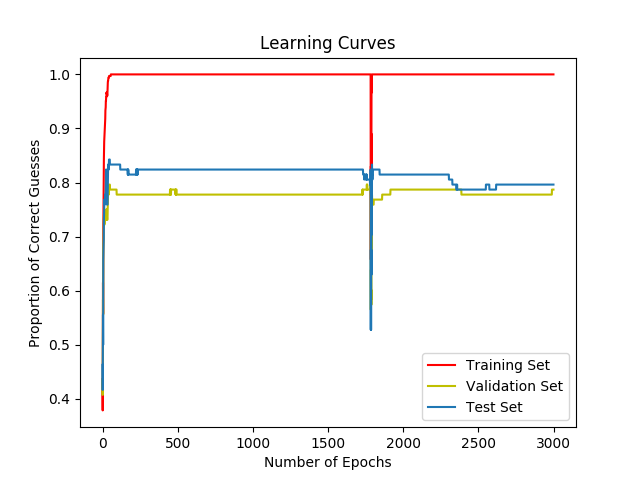
\includegraphics[width=\linewidth]{Part8LearningCurve.png}
		\caption{Learning curve for training, validation and test sets}
		\label{fig:pat8}
	\end{figure}

	We have used 60 images per actor for the training set, 20 images per actor for validation set and 20 images per actor for test set with the exception of Braccho where we have the proportional amount of images. We read each image, flatten the image and divide the pixel values by 255.0 so the input pixel values are between 0 and 1. We constructed the input matrix for each batch using vstack. We have initialized the weights to be close to 0. We used the xavier uniform distribution to initialize the weights.
	\begin{lstlisting}
	torch.nn.init.xavier_uniform(model[0].weight)
	\end{lstlisting}

	The activation function we used is ReLU. We used ReLU because it cheaper to compute than the other activation functions. Our model has one hidden layer, with 1024 neurons in the hidden layer. We used 64 X 64 X 3 cropped RGB images for the faces. To get the best performance, we have adjusted the number of neurons in the hidden layers, the batch size and number of epochs.


	\section{Part 9}
	Here are the two visualizations for actors Steve Carell and Angie Harmon.

	\begin{figure}[H]
		\centering
		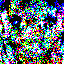
\includegraphics[width=0.5\linewidth]{Part9-Carell.png}
		\caption{Steve Carell Visualizations}
		\label{fig:part9}
	\end{figure}

	\begin{figure}[H]
		\centering
		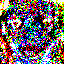
\includegraphics[width=0.5\linewidth]{Part9-Harmon.png}
		\caption{Angie Harmon}
		\label{fig:part9}
	\end{figure}

	We selected the units by selecting the indices of the output layer that correspond to the highest values which are more likely to be active part of the picture.

	\section{Part 10}

	\textbf{Description}
	First we modified AlexNet by removing all the layers after "conv4". Then we feed the images into the AlexNet one by one and flattened the activation values. Then we takes these values and use them as the inputs to train a neural network similar to the one we used in Part 8. The performance of the system which is around $96\%$ on the Test Set and $90\%$ on the validation set. The number of features we used to feed into the neural network is 43 264, which is the dimension of output of the AlexNet. The dimension of hidden units is 50. Like Part 8, we used ReLU as the activation function and we used the Xavier uniform distribution to initialize the weights.

	\begin{figure}[H]
		\centering
		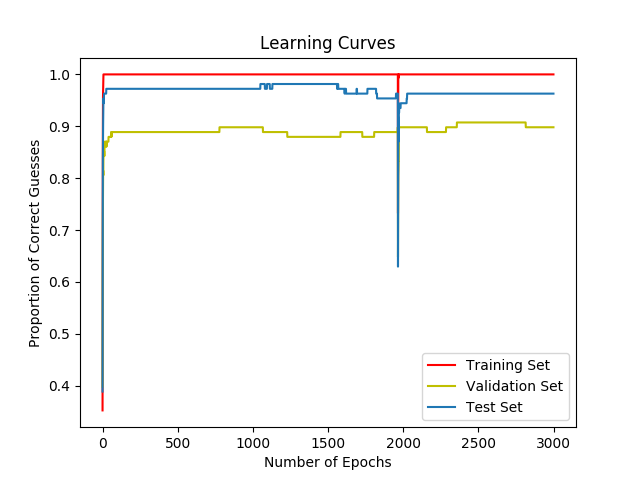
\includegraphics[width=\linewidth]{Part10LearningCurve.png}
		\caption{Learning Curve Part 10}
		\label{fig:part9}
	\end{figure}
\end{document}
